\section{Features}

When classifying entire neighborhoods, it is common for studies to use
a combination of features for the classification between formal and informal.
Our research will use methods for feature extraction that performed well in
previous research \cite{graesser2012image}. The methods used are: the Histogram
of Oriented Gradients, Line Support Region features and Linear Feature
Distribution. Both the Histogram of Oriented Gradients and Line Support Regions
are already implemented in a framework created by Jordan Graesser. This
framework is a python library, called spfeas, that is based on the
research Graesser et al conducted on the classification of formal and informal
settlements \cite{graesser2012image}. In addition to the features provided by
spfeas, this research will implement a new feature that measures the density of
road intersections in a given area, with the belief that area's with many
intersections are less likely to be informal.



% critique graesser

\subsection{Histogram of Oriented Gradients}
The spatial distribution of buildings in formal and informal settlements varies
significantly. The placement of houses in formal settlements are often placed
in a regular pattern with fixed orientations. Informal settlements, in
contrast, usually constructed without a design or regular pattern. This
difference in regularity is a characteristic that will be used
for classification of formal or informal settlements.

The order of regularity of an area can be captured using the number of
orientations in which buildings are constructed. Few orientations suggest
a formal settlements while many orientations suggest informal. The orientations
of buildings are calculated using the gradients returned by the application of
a sobel filter on the image. The gradients are quantized into a set of
orientations or bins. This results in a histogram commonly named the Histogram
of Oriented Gradients (HoG). High peaks the HoG correspond to a multitude of
similar gradients, thus uniformity in the image. Since uniformity is linked
to formal settlements, high peaks in the histogram correlate with formal
settlements. The informal settlements, on the other hand, are characterized by
the absence of peaks in the HoG due to the multitude of different gradients
caused by the irregular placement of buildings.

The HoG itself cannot reasonably be used as a feature, therefore the properties
of its distribution are used instead. One property of the HoG that well defines the
difference between formal and informal are the heaved central-shift moments.
The heaved central-shift moments are a method for the calculation of the
weighted mean of a histogram for any order.  The orders correspond to the
impact that high peaks in the histogram have on the mean. 


Histogram of Oriented Gradients
that characterize a certain area.


% praktisch hoe het hier gedaan is



\subsection{Line Support Region Features}

The formality of neighborhoods can be determined by observing the spatial
distribution of neighborhoods. In the same manner as HoG characterized
neighboorhoods by the orientation its buildings, neighborhoods, alternatively,
can be characterized by the size of their buildings. Informal settlements
generally lack the precence of large buildings in contrast with formal
settlements. The size of constructions can be characterised using the Line
Support Region (LSR) features \cite{unsalan2004classifying}. Likewise to HoG, LSR utilizes gradients
calulated from remote sensing imagery. LSR uses the fact that perfectly
straight lines have uniform gradients. In practice however, photographs never
contain perfectly straight lines, which results in similar but non uniform
gradients of lines. Therefore, LSR uses groups similar gradients to represent
a line in images to detect semi straight lines in images \cite{burns1986extracting}.




\section{Road Intersection Density}

In this field of study, as we have discussed, there exist many methods for characterizing image regions on land use. In some of these methods, the road network is used to try to classify regions, for instance, using road accessability metrics \cite{owen2013approach}. Using the road network to classify between different types of land use seems a promising approach to detect slums. We aim to extract the properties of the road network using a new strategy by detecting the road intersections in the image. This is based on the hypothesis that the density of the road intersections translates to the density of the road network, which is different for various types of neighborhoods. In our case, slums are visually and spatially distinct from surrounding building types, which could infer a difference in the road network density. Extracting density from the road intersections might therefore allow us to differentiate slums from their surroundings. In the next sections, we will discuss the various approaches we have used in the extraction of intersections for satellite images.



\subsection{Convolutional Neural Network}

Road detection and extraction from satellite images is well established field of study with a large variety of developed methods \cite{mena2003state}.  The specific detection of road intersection is less studied although there are studies covering the subject \cite{hu2007road} \cite{koutaki2004automatic} as part of general road network extraction. Since there exists a base of research in this field, we can use established methods to extract the road network, which can consequently be used as a basis for the extraction of the road intersections. 
A promising approach in road extraction is the use of Neural Networks \cite{mangala2011extraction} \cite{mokhtarzade2007road}. A study from 2017 was able to extract both the road network together with buildings with high accuracy using a Convolutional Neural Network \cite{alshehhi2017simultaneous}. We used the same approach although with a separate implementation of the convolutional neural network since the research paper did not include the software and data that was used in the study \cite{airs}. This implementation included a open-source set of images, that was designed for the training and validation of the neural network \cite{MnihThesis}. After training on the provided images, the network was tested on our own satellite images, resulting in erroneous predictions as it did not represent the road network in the provided image. The suspected cause of this failure is the difference in the training data to our satellite imagery data. The trainingset that was used contained satellite images obtained from mostly rural area's of the state of Massachusetts in the United States, while the data used in our research is from Bangalore in India which is mostly urban. The geographical features and the road systems presented in the two locations appears to be rather different, which could be a probable cause for the inability of the neural network to recognize the road network in Bangalore. Furthermore, the difference in resolutions of the two image sets could be another cause as the images of Massachusetts were of quite a lower resolution than the images of Bangalore.

\subsection{Hough Transform}
As an alternative to the neural network, we attempted to extract road networks using image processing techniques, which uses a number of operations resulting in a prediction of the road network. The first operation is the transformation of the RGB image to grayscale values, which is in preparation for Otsu's method for threshold, which is able to separate buildings from roads \cite{otsu1979threshold}. The resulting image, displayed in Figure \ref{fig:roads_hough}, is the predicted road network in the satellite image, where the white regions are detected as road. 

From an aerial point of view, the properties of roads are often elongated thin lines with constant width, and are often not possessed by other types of structures in images. We therefore detect these lines as roads using a Hough transform, which is able to extract straight lines from images and create mathematical definition of the lines \cite{duda1972use}. Once the roads are mathematically defined, determining the location of the intersection is straightforward.

\begin{figure}
\begin{tabular}{cc}
  \subfloat{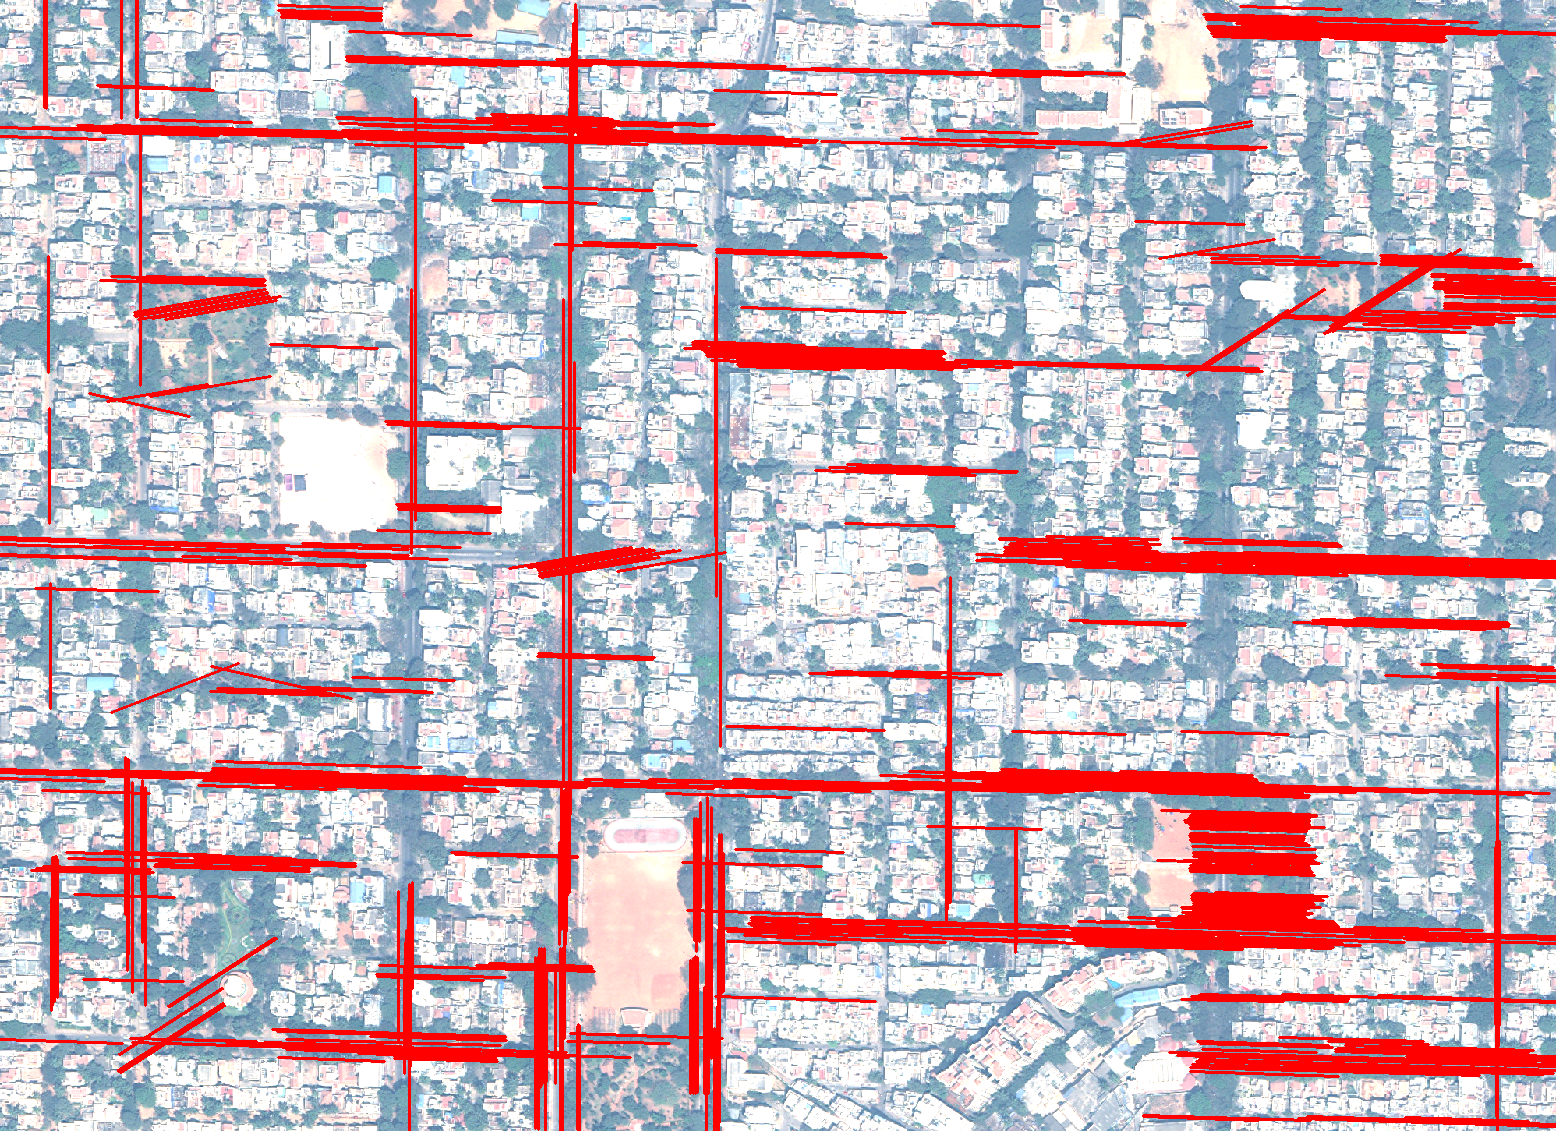
\includegraphics[width=7cm]{images/hough_road_section_8}}&
  \subfloat{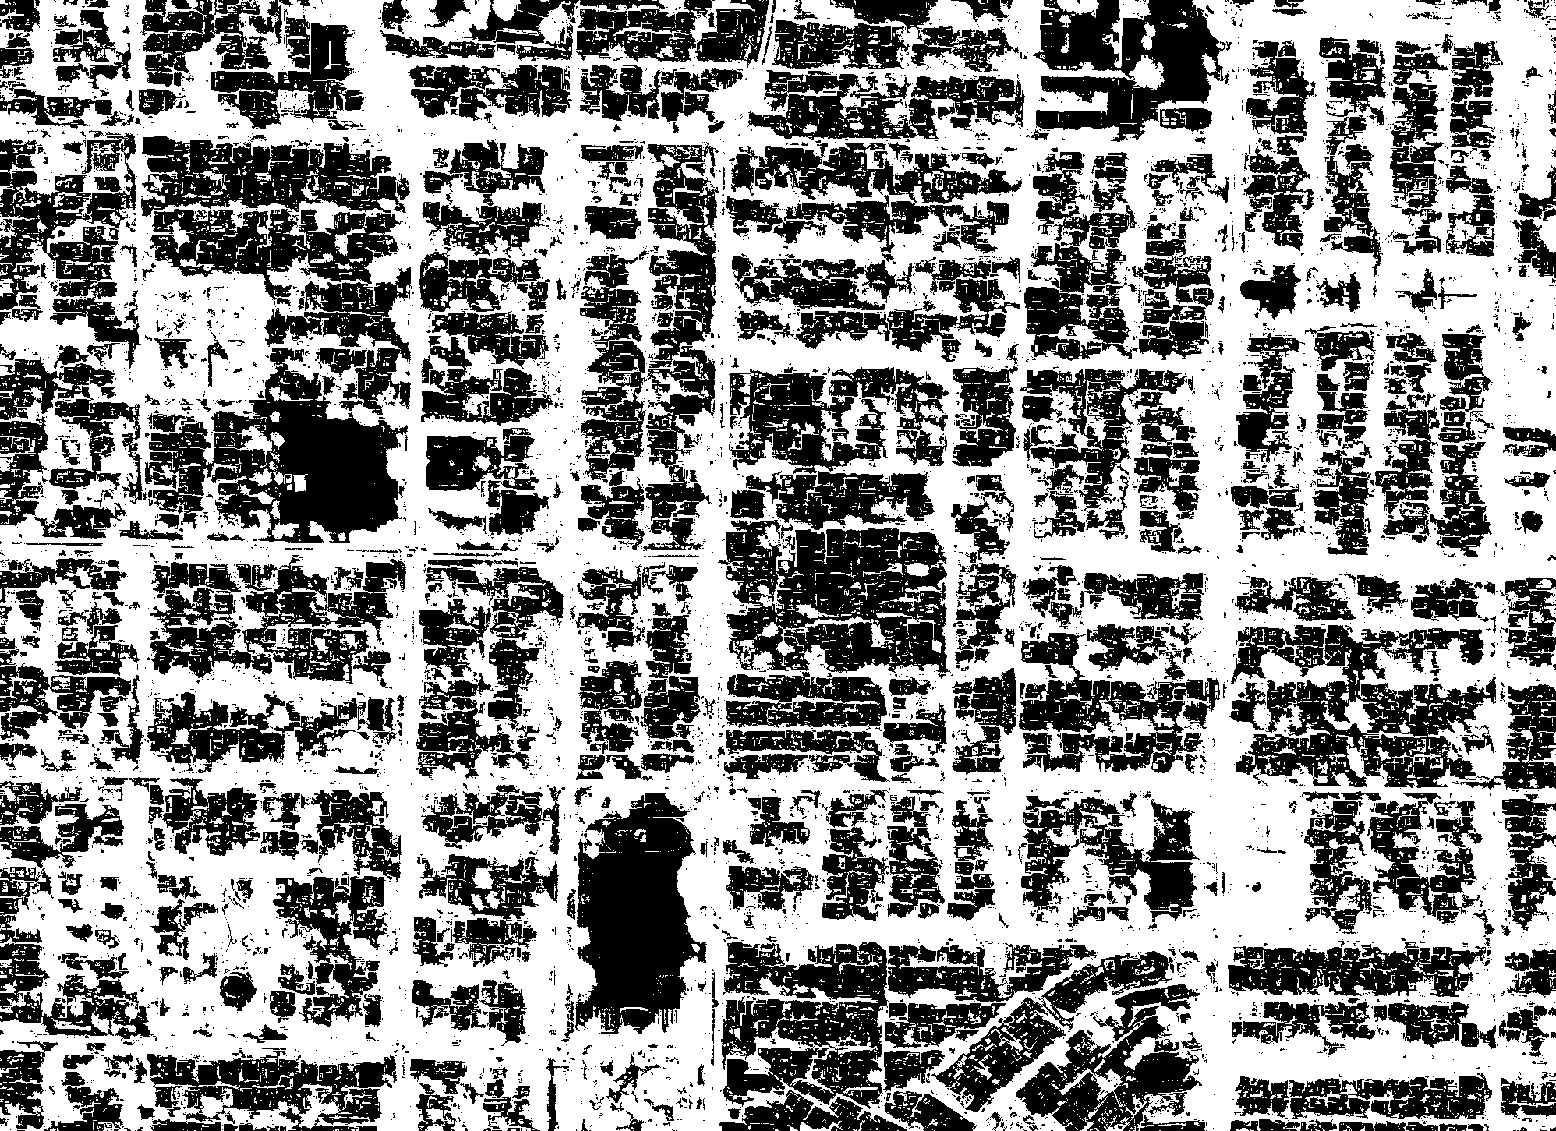
\includegraphics[width=7cm]{images/hough_road_section_8_mask}}
\end{tabular}
\caption{Detected roads using Otsu's thresholding method (left) combined with
Hough Transform (right)}
\label{fig:roads_hough}
\end{figure}

This method for road intersection detection was implemented in Python, resulting in a predicted road network and detected Hough lines displayed in Figure \ref{fig:roads_hough}. This was the most balanced results were able to achieve after changing the parameters for the creation of the prediction mask and Hough lines; different parameters would drastically increase recall and decrease accuracy beyond useful application. In this case, in contrast to the neural network, the extracted mask represents the road network quite accurately although the hough transform resulted in a lot of duplicate lines and noise. Even though the noise might be filtered out, we decided to pursuit a different method of intersection extraction. 

\subsection{Road Intersection Convolution}
In contrast to the original approach that first extracts the road network followed with the to detection of the intersections, we changed the approach of intersection detection to directly extract intersections from the satellite image. In our new approach, we apply a convolution using a kernel in the shape of an cross directly on the satellite image. Because the kernel matches the shape of an intersection, the output of the convolution will have peaks in the output image on the positions of the intersections. The results from the proof of concept are displayed in Figure \ref{fig:roads_conv}.
This approach is partly based on previous research; it has similarities to the use footprints to find the direction of intersections \cite{hu2007road}. The footprint approach uses certain points, called seeds, in the image from where the road network expands using road segments. These road segments can be one of a few classes, for example, a straight road, T junction and cross intersection. The type depends on its surrounding pixels, which form a footprint that is classified as either one of the listed classes. Another study used a similar approach, which explicitly displays the different sizes of intersections \cite{koutaki2004automatic}. However, these two studies do not use convolution but different methods to match the footprints to the intersections in the image. Our method does not have to be as complicated because the orientation of an intersection is not important in our case, only the location is required.

\begin{figure}
	\begin{tabular}{cc}
		\subfloat{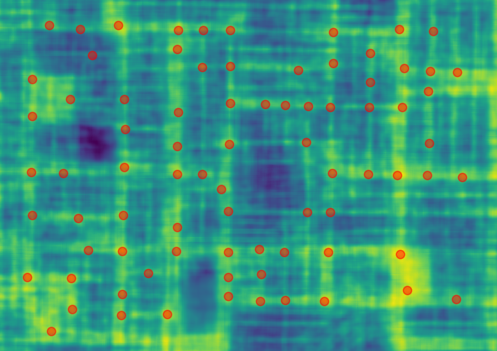
\includegraphics[width=7cm]{images/conv_road_section_8_1}}&
		\subfloat{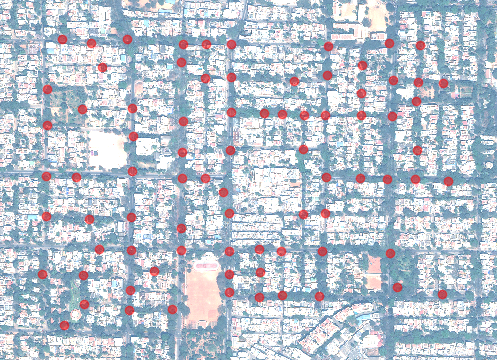
\includegraphics[width=7cm]{images/conv_road_section_8_2}}
	\end{tabular}
	\caption{Detection of intersections using convolution of a cross shaped kernel.
		Left: Heatmap of output of the convolution; Right: Located peaks overlayed on input image}
	\label{fig:roads_conv}
\end{figure}

Preceding the convolution, the satellite image is transformed to grayscale and subsequently inverted in color. In certain areas, the grayscale version of the image will already have a large contrast between roads and the surrounding buildings. However, this not true for the sections displayed in Figure \ref{fig:sections}. We therefore apply the Otsu's thresholding is after the transformation to grayscale, which results in a black and white version of the image with a large contrast between roads and buildings. 

The original kernel that was used as proof of concept is a n by n matrix, containing a cross of ones
with the remainder filled with zero's, as illustrated in Figure \ref{fig:conv_kernel}a on the left. To clarify some terminology, the toe of an intersection is one of the roads leading to the
intersection. In the case of Figure \ref{fig:conv_kernel}a, there are four toes
with a width and length two and three matrix cells, respectively. The width and length of a toe will also be referred to as the road width and length respectively. Theoretically, this kernel has the optimal activation when it is exactly placed on the same shape of the kernel, thus the shape of a cross intersection. It is therefore important to match the shape of the kernel to the shape of the intersections in the image, which means that the width of the toe in the kernel depends on the road width of the intersections in the image. Therefore, the dimension of the kernel depends on the image used and the scale of the image. In practice, the kernel will be much larger than the kernel in Figure \ref{fig:conv_kernel}a as the road width and length are generally in the dozens rather than the single digits.

\begin{figure}%	
	\centering
	\begin{tabular}{cc}	
		{$\displaystyle
			\begin{pmatrix}
			0 & 0 & 0 & 1 & 1 & 0 & 0 & 0\\
			0 & 0 & 0 & 1 & 1 & 0 & 0 & 0\\
			0 & 0 & 0 & 1 & 1 & 0 & 0 & 0\\
			1 & 1 & 1 & 1 & 1 & 1 & 1 & 1\\
			1 & 1 & 1 & 1 & 1 & 1 & 1 & 1\\
			0 & 0 & 0 & 1 & 1 & 0 & 0 & 0\\
			0 & 0 & 0 & 1 & 1 & 0 & 0 & 0\\
			0 & 0 & 0 & 1 & 1 & 0 & 0 & 0
			\end{pmatrix}
			$} &
		$\vcenter{\hbox{
\includegraphics[width=4cm]{images/gauss_kernel}}}$\\
		a) Simple convolution kernel & b) Gaussian convolution kernel
	\end{tabular}
	
	\caption{Different convolution kernels}%
	\label{fig:conv_kernel}
\end{figure}

Figure \ref{fig:roads_conv} displays the results of the convolution and the corresponding location of the detected peaks. The image used was a small section of the satellite image of Bangalore, not to be confused with the other three sections. This specific region was chosen because of the width of the roads and the regularity of the road network with 90 degree angles between the toes of the intersection. Furthermore, the horizontal and vertical roads run parallel to the edges of the image. The road network is also quite distinct from the background despite the vegetation covering large part of the roads, which might actually increase the contrast between the road and the surroundings.

The peaks, displayed as red dots, are located using local maxima detection from the Python scikit-image package \cite{scikit-image}. This function detects local maxima in an image, which are regions that stand out from surrounding values. 

\subsubsection{Kernels}
In the development of this method, we have designed a number of kernels to extract road intersections from images. In order to increase accuracy of the detected intersections, we created a new type of kernel that is similar to the kernel displayed in Figure \ref{fig:conv_kernel}a, but with the zero's replaced by negative numbers. The distance from the cross is proportional to the negative value of a cell in the kernel. When applied to areas which are not an intersection, the negative cells of the kernel should produce a large negative activation. In practice, this kernel seems to be activated by intersection as well as straight sections of road, which introduces many false positives.

To account for different widths of roads in an image, we created a kernel using Gaussian distributions, displayed in Figure \ref{fig:conv_kernel}b. This kernel should smooth the contrast between roads and roadside and might remove noise. This kernel counts the center of the road the most while the edges
of the road count for less. This should increase the scalability of the kernel to multiple types and sizes of roads, such as alleys or main streets. The Gaussian kernel will therefore used for experiments on the three image sections.

\subsubsection{Intersection Detection Evaluation}

\begin{figure}
\begin{tabular}{cc}
  \subfloat{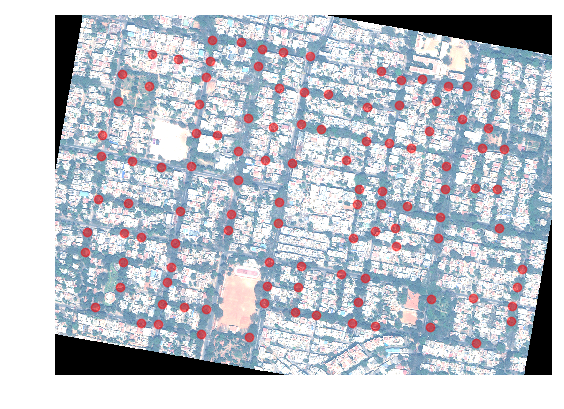
\includegraphics[width=7cm]{images/rot10}}&
  \subfloat{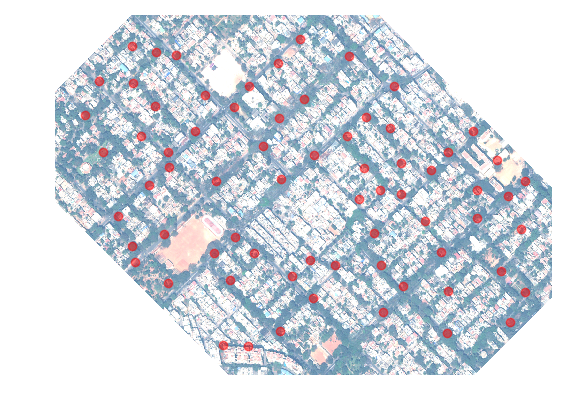
\includegraphics[width=7cm]{images/rot45}}
\end{tabular}
\caption{Performance of intersection detection in rotated intersections, from
  left to right with 10 and 45 degrees respectively}
\label{fig:roads_rot}
\end{figure}

A fundamental problem of this approach is the relation between the kernel and the resolution of the image. An increase of the scale or resolution of an image will change the dimensions of the intersections, thus requiring a change to the content of the kernel. Although the Gaussian distribution should increase scalability, it is still largely required to adjust parameters according to the resolution of the image.\newline

\noindent
Because of the fixed orientation of the cross in the kernel, this approach should inherently be prone to differences in orientation. In the proof of concept, we explicitly used a road system with a constant orientation, as displayed in Figure \ref{fig:roads_conv}. The constant orientation of the intersections, enable the kernel to correctly detect a large number of intersections. In many other areas, the road system is not nearly as consistent, for instance ,the sections displayed in Figure \ref{fig:sections}. Intersections that are rotated relative to the orientation of the kernel should therefore be more difficult to detect. To test this hypothesis, we performed the intersection detection under rotations of 10 and 45 degrees, as displayed in Figure \ref{fig:roads_rot}. It seems that, under slight rotation, the fast majority of intersections are still detected whereas increasing the rotation to the maximum of 45 degrees results in a loss of many detections. Interestingly enough, there is almost no increase in false positives. It might be that this seemingly invariance to rotation is caused by the method of peaks detection.  When using a rotated image, the resulting convolution is more smooth with less peaks compared to the original image. It seems that the local maxima detection is still able to correctly detect these faint peaks in the convoluted image. Nevertheless, this approach should primarilty be used for images with minimal rotation since this produces the most correct detections.\newline

\noindent
The road system displayed in figures \ref{fig:roads_conv} and \ref{fig:roads_rot} do not well represent the general road network encountered in the whole of the satellite image. This becomes apparent when observing the road system in the three section displayed in Figure \ref{fig:sections}. Although the majority of land area in these sections is formal, there is a clear contrast between these road systems and the road system used in the development of this feature. The road system in the three sections are much more narrow, shorter, and less regular than the road system in \ref{fig:roads_conv}. In these sections, on many occasions, even manual extraction of intersections is quite difficult. It is, for instance, often not clear whether the space between two buildings is an empty strip of land or actually a road. 

%Due to the different nature of the road systems, parameters used to detect the intersections in Figure \ref{fig:roads_conv} and the sections in Figure \ref{fig:sections} are different. Because the streets in these three sections are generally more narrow and less long, both the road width and road length parameters are decreased relative to the parameters used in Figure \ref{fig:roads_conv}. Furthermore, the parameters for the local maxima detection are changed to only detect peaks that are really distinct from their surroundings. The motivation behind this is to reduce noise introduced by the irregularity and obscurity of the road network.

We could not perform a objective evaluation of the intersection detection due to the lack of a ground truth of the road intersections. Since we are not in the possession of a ground truth, we cannot calculate objective measures of detection performance, such as accuracy, recall and the F1 score. Instead, the performance evaluation of the various methods and parameters used for the detection of intersection is based on visual observation.

In conclusion, the use of a cross shaped kernel together with convolution seems to be able to extract the location of road intersections quite well. Although, for real world applications, such as road system mapping, this method for intersection detection might not be sophisticated enough, since this method does not include the direction of the intersection. Furthermore, false positives and negatives are quite prevalent using this approach; it might meet not the performance achieved by different methods.

\subsection{Feature extraction}

\begin{figure}
	\begin{tabular}{cc}
		\subfloat{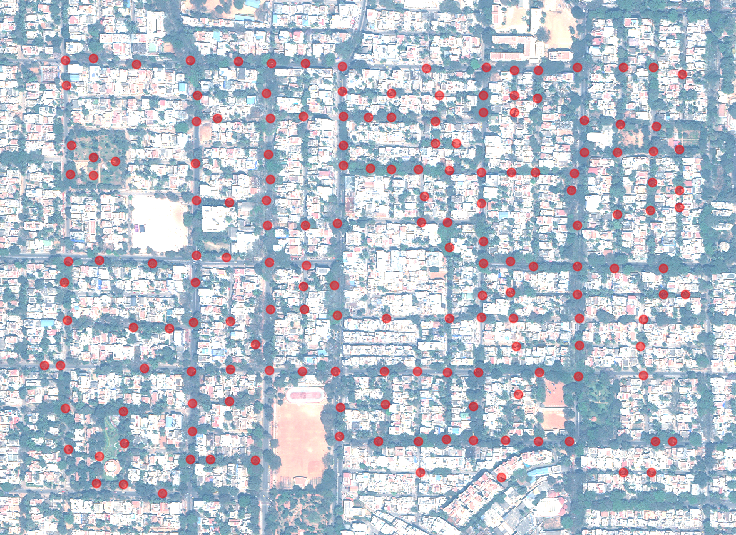
\includegraphics[width=7cm]{images/hotspotint}}&
		\subfloat{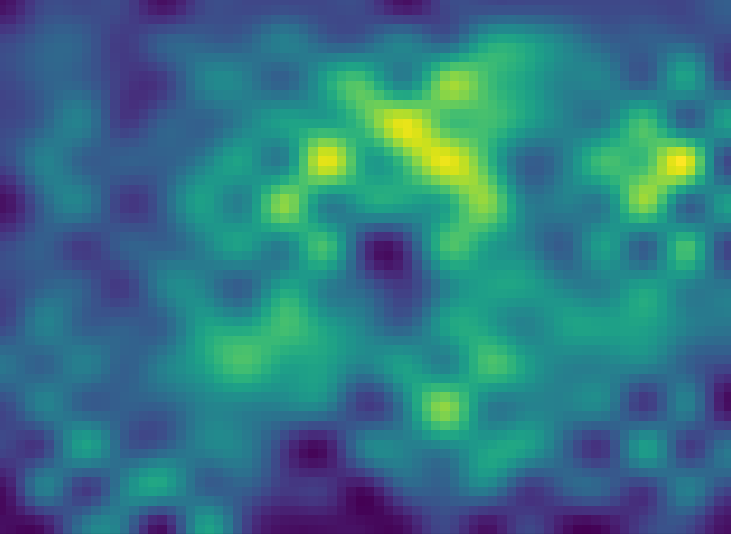
\includegraphics[width=7cm]{images/hotspot}}
	\end{tabular}
	\caption{Hotspots extracted from the detected intersections. Left: Detected road intersections; Right: Resulting hotspot map of the local G function}
	\label{fig:roads_hotspot}
\end{figure}


The positions of the road intersections extracted from the image are used to create a intersection density map of the area. The density of road intersections in an area is measured using spatial statistics provided by the Getis and Ord's local G function \cite{getis1992analysis}. The local G function is a measure of spatial association between spatially distributed data. In our case, this data is the locations of the intersections in the image. The local G function is able to detect local hotspots and coldspots in instance data, effectively indicating the location of hotspots and coldspots in the density of intersections in the image of interest.

\begin{figure}[h]
	\centering
	$ \mathlarger{\mathlarger{\mathlarger{ G_i(d) = \frac{\sum\limits_{j=1}^{n}w_{ij}(d)x_j}{\sum\limits_{j=1}^{n}x_j} }}} $
	\caption{Definition of the local G function}
	\label{g_function}
\end{figure}


The formula of the Getis-Ord local G function $G_i(d)$ is displayed in Figure \ref{g_function}, which defines for a data point $i$ on a Cartesian plane a ratio using the neighboring data points within a radius $d$. In our case, $i$ is the location of an intersection, with $d$ being the scale of the feature. Regarding the variables in the numerator of the fraction, $n$ is the total number of data points, $j$ is every data point that is not $i$, $w_ij{d}$ is a function that returns zero or one whether $j$ is within the radius $d$ of $i$, and $x_j$ specifies the weight of $j$. The enumerator sums up all weights $x_j$ of the data points within the radius $d$ of $i$. In our case, when using the location of road intersections, we do not have weights other than ones. However, because we rasterize the locations of the intersections to a grid in the shape of the HoG and LSR features, the weights will indicate the number of intersections that fell within a certain block in the grid. The denominator is the sum of the weights of all data points, regardless of their location. This fraction is in essence a ratio between the points within the radius of $i$ and all points. 

\begin{figure}[h]
	\centering
	$ \mathlarger{\mathlarger{\mathlarger{ z = \frac{x - \mu}{\sigma} }}} $
	\caption{Definition of the Z score}
	\label{z_score}
\end{figure}

We use the ratios created by $G_i(d)$ to create a statistical feature using the Z score. This score is calculated using the formula displayed in Figure \ref{z_score} where $x$ is the $G_i(d)$, $\mu$ is the mean and $\sigma$ the standard deviation of all $G_i(d)$ \cite{kreyszig2010advanced}. The Z score is a form of outlier detection, where negative and positive scores indicate a deviation from the mean. Using the Z score, we can detect hot and cold spots in the $G_i(d)$ ratios, and therefore detect hotspots and cold spots in the density of road intersections. The exact calculation of the Z score for the local G function with definitions of the $G_i(d)$ mean and variance can be found in the paper\cite{getis1992analysis}. The Z score applied to local G function results in a map of hotspots and cold spots of the road intersections, as illustrated by Figure \ref{fig:roads_hotspot}.

Both the local G function and Z score are implemented in the PySal Python packackage \cite{rey2010pysal}. The resulting map from the local G function and Z score is used as a feature and will be referred to as the \textit{Road Intersection Density} or RID for short.





